% enstitü adı ortalanmadıysa itutez.cls içinde "%% shift right" arayın.
\documentclass[onluarkali,ingilizce,doktora,bez,LisansustuEgitim]{itutez}

% bu dosya böylece kalabilir.
%!TEX root = ../tez.tex
\usepackage{cite}
\usepackage{amsmath,amsthm}
\usepackage{mathtools}
\usepackage{tikz}
\usepackage{graphicx}
\usepackage{multirow}

\font\tenipa=tipa10
\def\schwa{{\tenipa\char64}}

\graphicspath{{figures/}}


\usepackage{color}
\usepackage{times}
\usepackage{amssymb,mathptmx,amsbsy,bm}
\usepackage{caption}
\usepackage{graphics}
\usepackage{wrapfig}
\usepackage{epsfig}
\usepackage{enumerate}
\usepackage{rotating}
\usepackage{colortbl}
\usepackage{pstricks}
\usepackage{pst-plot}
\usepackage{latexsym}
\usepackage{rotating}


% ihtiyaç duyduğunuz paketleri ve komutları bunun içine yazın.
% maksat kodlar temiz görünsün.

\newtheorem{theorem}{Theorem}[chapter]
\newtheorem{lemma}[theorem]{Lemma}
\newtheorem*{remark}{Remark}

\newtheorem{corollary}[theorem]{Corollary}
\newtheorem{proposition}[theorem]{Proposition}

\theoremstyle{definition}
\newtheorem{definition}[theorem]{Definition}
\newtheorem*{example}{Example}
\newtheorem*{notation}{Notation}

% bu dosyanın içini doldurun.

% Soyadı BÜYÜK harfle.
\yazar{Name}{SURNAME} 
\ogrencino{702082003}

% Unvan yazmak zorunlu. Aşağıdaki gibi parantez içinde.
\unvan{(Any Profession)}

% Enstitü sitesinden bakın, yanlış olmasın.
\anabilimdali{Matematik Mühendisliği Anabilim Dalı}{Department of Mathematical Engineering}
\programi{Matematik Mühendisliği Programı}{Mathematical Engineering Programme}

% Tezin savunulduğu ay ve yıl. Aşağıdaki gibi büyük küçük harfe dikkat.
\tarih{HAZİRAN 2022}{JUNE 2022}
\tarihKucuk{Haziran 2022}{June 2022}

% Tez hocanız yani
\tezyoneticisi{Prof. Dr. John DOE}{Istanbul Technical University}   

% Tez başlığı üç satıra sığmalı. Bence iki satır güzel görünüyor.
\baslik{BAŞLIK İLK SATIR}{GEREKLİYSE İKİNCİ SATIR}{GEREKLİYSE ÜÇÜNCÜ SATIR}
\title{TITLE FIRST LINE}{SECOND LINE IF NECESSARY}{THIRD LINE IF NECESSARY}

% Tez sunuş formunu doldurup gönderdikten sonra,
% "Tez savunma jürisi bildirim yazısı" konulu emailde,
% "Yönetim kurulu tarihi" yazan kısım tez verme tarihi oluyor.
\tezvermetarih{3 Haziran 2022}{3 June 2022}
\tezsavunmatarih{22 Haziran 2022}{22 June 2022}

% varsa eş danışmanı. Ve jüriler.
\esdanismani{}{}   
\juriBir{Prof. Dr. Johann Sebastian BACH}{X University}
\juriIki{Prof. Dr. Wolfgang Amadeus MOZART}{Y University}
\juriUc{Assoc. Prof. Dr. Ludwig van BEETHOVEN}{Z University}
\juriDort{Asst. Prof. Dr. Frédéric CHOPIN}{T University}
\juriBes{}{}


% Hiç kimseyi bulamıyorsanız Gauss'a ithaf edin tezinizi.
\ithaf{Dedication...}

% Önsözde emeği geçen herkese teşekkür ediyoruz, mesela bana.
\onsoz{For the foreword, 1 line spacing must be set. The foreword, written
as a first page of the thesis must not exceed 2 pages. The 
acknowledgements must be given in this section.
After the foreword text, name of the author (right-aligned), and
the date (as month and year) must be written (left-aligned). Surnames should be capitalized. These two expressions must be in the same line. The foreword is written with 1 line spacing. } % 
\kisaltmalistesi{\hspace{-3mm}
\begin{tabular}{p{2cm}l}
{\bf{AIC}} & {\bf:} Akaike Information Criteria\\
{\bf ANN} & {\bf:} Artificial Neural Network\\
{\bf App} & {\bf:} Appendix\\
{\bf BP} & {\bf:} Backpropagation\\
{\bf CGI} & {\bf:} Common Gateway Interface\\
{\bf ESS} & {\bf:} Error sum-of-squares\\
{\bf GARCH} & {\bf:} Generalized Autoregressive Conditional Heteroskedasticity\\
{\bf GIS} & {\bf:} Geographic Information Systems\\
{\bf HCA} & {\bf:} Hierarchical Cluster Analysis\\
{\bf Mbps} & {\bf:} Megabits\\
{\bf St} & {\bf:} Station\\
{\bf SWAT} & {\bf:} Soil and Water Assessment Tool\\
{\bf UMN} & {\bf:} University of Minnesota\\
\end{tabular}

}
\sembollistesi{\hspace{-3mm}
\begin{tabular}{p{2cm}l}
{\bf{C}} & {\bf:} Capacitance\\
{\bf H} & {\bf:} The amount of heat\\
{\bf M\textsubscript{x},} {\bf M\textsubscript{y}} & {\bf:} Torque Components\\
{\bf N\textsubscript{x},} {\bf N\textsubscript{y},} {\bf N\textsubscript{z}} & {\bf:} Normal Power Components\\
{\bf q} & {\bf:} Phase load\\
{\bf t} & {\bf:} Time\\
{\bf u, v} & {\bf:} Displacement Vector Components\\
{\bf w} & {\bf:} Angular velocity\\
{\bf XC} & {\bf:} Capacitive reactance\\
{\bf XL} & {\bf:}  Inductive reactance\\
%{\bf {\textalpha}} & {\bf:} Asal gerilme do\u{g}rultusundan sapma a\c{c}\i s\i\\
%{\bf {\textrho}} & {\bf:} Yo\u{g}unluk\\
%{\bf {\textsigma\textsubscript{x},}} {\bf {\textsigma\textsubscript{y},}} {\bf {\textsigma\textsubscript{xy}}} & {\bf:} Kabuk i\c{c} gerilmeleri\\
\end{tabular}

}

% Özeti güzel yazın keyifle okuyalım.
\ozet{1 line spacing must be set for summaries. For theses in Turkish, the summary in Turkish must have 300 words minimum and span 1 to 3 pages, whereas the extended summary in English must span 3-5 pages.

For theses in English, the summary in English must have 300 words minimum and span 1-3 pages, whereas the extended summary in Turkish must span 3-5 pages.

A summary must briefly mention the subject of the thesis, the method(s) used and the conclusions derived.

References, figures and tables must not be given in Summary.

Above the Summary, the thesis title in first level title format (i.e., 72 pt before and 18 pt after paragraph spacing, and 1 line spacing) must be placed. Below the title, the expression ÖZET (for summary in Turkish) and SUMMARY (for summary in English) must be written horizontally centered.

It is recommended that the summary in English is placed before the summary in Turkish.


Lorem ipsum dolor sit amet, consectetur adipiscing elit. Praesent imperdiet, nisi 
nec aliquam cursus, dui turpis mollis nisl, ac consequat tellus sapien sit amet 
magna. Duis vel venenatis velit. Vestibulum ante ipsum primis in faucibus orci 
luctus et ultrices posuere cubilia Curae; Proin malesuada risus nec metus dapibus 
eu tincidunt lectus dignissim. 

Lorem ipsum dolor sit amet, consectetur adipiscing elit. Praesent imperdiet, nisi 
nec aliquam cursus, dui turpis mollis nisl, ac consequat tellus sapien sit amet 
magna. Duis vel venenatis velit. Vestibulum ante ipsum primis in faucibus orci 
luctus et ultrices posuere cubilia Curae; Proin malesuada risus nec metus dapibus 
eu tincidunt lectus dignissim. 

Lorem ipsum dolor sit amet, consectetur adipiscing elit. Praesent imperdiet, nisi 
nec aliquam cursus, dui turpis mollis nisl, ac consequat tellus sapien sit amet 
magna. Duis vel venenatis velit. Vestibulum ante ipsum primis in faucibus orci 
luctus et ultrices posuere cubilia Curae; Proin malesuada risus nec metus dapibus 
eu tincidunt lectus dignissim. 

Lorem ipsum dolor sit amet, consectetur adipiscing elit. Praesent imperdiet, nisi 
nec aliquam cursus, dui turpis mollis nisl, ac consequat tellus sapien sit amet 
magna. Duis vel venenatis velit. Vestibulum ante ipsum primis in faucibus orci 
luctus et ultrices posuere cubilia Curae; Proin malesuada risus nec metus dapibus 
eu tincidunt lectus dignissim. 

Lorem ipsum dolor sit amet, consectetur adipiscing elit. Praesent imperdiet, nisi 
nec aliquam cursus, dui turpis mollis nisl, ac consequat tellus sapien sit amet 
magna. Duis vel venenatis velit. Vestibulum ante ipsum primis in faucibus orci 
luctus et ultrices posuere cubilia Curae; Proin malesuada risus nec metus dapibus 
eu tincidunt lectus dignissim. 

Lorem ipsum dolor sit amet, consectetur adipiscing elit. Praesent imperdiet, nisi 
nec aliquam cursus, dui turpis mollis nisl, ac consequat tellus sapien sit amet 
magna. Duis vel venenatis velit. Vestibulum ante ipsum primis in faucibus orci 
luctus et ultrices posuere cubilia Curae; Proin malesuada risus nec metus dapibus 
eu tincidunt lectus dignissim. 
Lorem ipsum dolor sit amet, consectetur adipiscing elit. Praesent imperdiet, nisi 
nec aliquam cursus, dui turpis mollis nisl, ac consequat tellus sapien sit amet 
magna. Duis vel venenatis velit. Vestibulum ante ipsum primis in faucibus orci 
luctus et ultrices posuere cubilia Curae; Proin malesuada risus nec metus dapibus 
eu tincidunt lectus dignissim. 

Lorem ipsum dolor sit amet, consectetur adipiscing elit. Praesent imperdiet, nisi 
nec aliquam cursus, dui turpis mollis nisl, ac consequat tellus sapien sit amet 
magna. Duis vel venenatis velit. Vestibulum ante ipsum primis in faucibus orci 
luctus et ultrices posuere cubilia Curae; Proin malesuada risus nec metus dapibus 
eu tincidunt lectus dignissim. 

Lorem ipsum dolor sit amet, consectetur adipiscing elit. Praesent imperdiet, nisi 
nec aliquam cursus, dui turpis mollis nisl, ac consequat tellus sapien sit amet 
magna. Duis vel venenatis velit. Vestibulum ante ipsum primis in faucibus orci 
luctus et ultrices posuere cubilia Curae; Proin malesuada risus nec metus dapibus 
eu tincidunt lectus dignissim. 

Lorem ipsum dolor sit amet, consectetur adipiscing elit. Praesent imperdiet, nisi 
nec aliquam cursus, dui turpis mollis nisl, ac consequat tellus sapien sit amet 
magna. Duis vel venenatis velit. Vestibulum ante ipsum primis in faucibus orci 
luctus et ultrices posuere cubilia Curae; Proin malesuada risus nec metus dapibus 
eu tincidunt lectus dignissim. 

Lorem ipsum dolor sit amet, consectetur adipiscing elit. Praesent imperdiet, nisi 
nec aliquam cursus, dui turpis mollis nisl, ac consequat tellus sapien sit amet 
magna. Duis vel venenatis velit. Vestibulum ante ipsum primis in faucibus orci 
luctus et ultrices posuere cubilia Curae; Proin malesuada risus nec metus dapibus 
eu tincidunt lectus dignissim. 

Lorem ipsum dolor sit amet, consectetur adipiscing elit. Praesent imperdiet, nisi 
nec aliquam cursus, dui turpis mollis nisl, ac consequat tellus sapien sit amet 
magna. Duis vel venenatis velit. Vestibulum ante ipsum primis in faucibus orci 
luctus et ultrices posuere cubilia Curae; Proin malesuada risus nec metus dapibus 
eu tincidunt lectus dignissim. 

Lorem ipsum dolor sit amet, consectetur adipiscing elit. Praesent imperdiet, nisi 
nec aliquam cursus, dui turpis mollis nisl, ac consequat tellus sapien sit amet 
magna. Duis vel venenatis velit. Vestibulum ante ipsum primis in faucibus orci 
luctus et ultrices posuere cubilia Curae; Proin malesuada risus nec metus dapibus 
eu tincidunt lectus dignissim. 

Lorem ipsum dolor sit amet, consectetur adipiscing elit. Praesent imperdiet, nisi 
nec aliquam cursus, dui turpis mollis nisl, ac consequat tellus sapien sit amet 
magna. Duis vel venenatis velit. Vestibulum ante ipsum primis in faucibus orci 
luctus et ultrices posuere cubilia Curae; Proin malesuada risus nec metus dapibus 
eu tincidunt lectus dignissim. 

Lorem ipsum dolor sit amet, consectetur adipiscing elit. Praesent imperdiet, nisi 
nec aliquam cursus, dui turpis mollis nisl, ac consequat tellus sapien sit amet 
magna. Duis vel venenatis velit. Vestibulum ante ipsum primis in faucibus orci 
luctus et ultrices posuere cubilia Curae; Proin malesuada risus nec metus dapibus 
eu tincidunt lectus dignissim. 

Lorem ipsum dolor sit amet, consectetur adipiscing elit. Praesent imperdiet, nisi 
nec aliquam cursus, dui turpis mollis nisl, ac consequat tellus sapien sit amet 
magna. Duis vel venenatis velit. Vestibulum ante ipsum primis in faucibus orci 
luctus et ultrices posuere cubilia Curae; Proin malesuada risus nec metus dapibus 
eu tincidunt lectus dignissim. 

Lorem ipsum dolor sit amet, consectetur adipiscing elit. Praesent imperdiet, nisi 
nec aliquam cursus, dui turpis mollis nisl, ac consequat tellus sapien sit amet 
magna. Duis vel venenatis velit. Vestibulum ante ipsum primis in faucibus orci 
luctus et ultrices posuere cubilia Curae; Proin malesuada risus nec metus dapibus 
eu tincidunt lectus dignissim. 

Lorem ipsum dolor sit amet, consectetur adipiscing elit. Praesent imperdiet, nisi 
nec aliquam cursus, dui turpis mollis nisl, ac consequat tellus sapien sit amet 
magna. Duis vel venenatis velit. Vestibulum ante ipsum primis in faucibus orci 
luctus et ultrices posuere cubilia Curae; Proin malesuada risus nec metus dapibus 
eu tincidunt lectus dignissim. 

Lorem ipsum dolor sit amet, consectetur adipiscing elit. Praesent imperdiet, nisi 
nec aliquam cursus, dui turpis mollis nisl, ac consequat tellus sapien sit amet 
magna. Duis vel venenatis velit. Vestibulum ante ipsum primis in faucibus orci 
luctus et ultrices posuere cubilia Curae; Proin malesuada risus nec metus dapibus 
eu tincidunt lectus dignissim. 

Lorem ipsum dolor sit amet, consectetur adipiscing elit. Praesent imperdiet, nisi 
nec aliquam cursus, dui turpis mollis nisl, ac consequat tellus sapien sit amet 
magna. Duis vel venenatis velit. Vestibulum ante ipsum primis in faucibus orci 
luctus et ultrices posuere cubilia Curae; Proin malesuada risus nec metus dapibus 
eu tincidunt lectus dignissim. }
\summary{1 line spacing must be set for summaries. For theses in Turkish, the summary in
Turkish must have 300 words minimum and span 1 to 3 pages, whereas the extended
summary in English must span 3-5 pages.
For theses in English, the summary in English must have 300 words minimum and
span 1-3 pages, whereas the extended summary in Turkish must span 3-5 pages.
A summary must briefly mention the subject of the thesis, the method(s) used and 
the conclusions derived.
References, figures and tables must not be given in Summary.
Above the Summary, the thesis title in first level title format 
(i.e., 72 pt before and 18 pt after paragraph spacing, and 1 line 
spacing) must be placed. Below the title, expression {\bf \"OZET} 
(for summary in Turkish) and {\bf SUMMARY} (for summary in English)
must be written horizontally centered.
It is recommended that the summary in English is placed before
the summary in Turkish.

Lorem ipsum dolor sit amet, consectetur adipiscing elit. Praesent imperdiet, nisi 
nec aliquam cursus, dui turpis mollis nisl, ac consequat tellus sapien sit amet 
magna. Duis vel venenatis velit. Vestibulum ante ipsum primis in faucibus orci 
luctus et ultrices posuere cubilia Curae; Proin malesuada risus nec metus dapibus 
eu tincidunt lectus dignissim. Morbi massa orci, luctus at vulputate lacinia, 
vestibulum sed libero. Ut accumsan tortor vulputate dolor semper id dignissim 
augue semper. Proin ac purus mi. 

Lorem ipsum dolor sit amet, consectetur adipiscing elit. Praesent imperdiet, nisi 
nec aliquam cursus, dui turpis mollis nisl, ac consequat tellus sapien sit amet 
magna. Duis vel venenatis velit. Vestibulum ante ipsum primis in faucibus orci 
luctus et ultrices posuere cubilia Curae; Proin malesuada risus nec metus dapibus 
eu tincidunt lectus dignissim. Morbi massa orci, luctus at vulputate lacinia, 
vestibulum sed libero. Ut accumsan tortor vulputate dolor semper id dignissim 
augue semper. Proin ac purus mi. 

Lorem ipsum dolor sit amet, consectetur adipiscing elit. Praesent imperdiet, nisi 
nec aliquam cursus, dui turpis mollis nisl, ac consequat tellus sapien sit amet 
magna. Duis vel venenatis velit. Vestibulum ante ipsum primis in faucibus orci 
luctus et ultrices posuere cubilia Curae; Proin malesuada risus nec metus dapibus 
eu tincidunt lectus dignissim. Morbi massa orci, luctus at vulputate lacinia, 
vestibulum sed libero. Ut accumsan tortor vulputate dolor semper id dignissim 
augue semper. Proin ac purus mi. } 

\begin{document}
%!TEX root = ../tez.tex
\chapter{INTRODUCTION}\label{introduction}

Lorem ipsum dolor sit amet, consectetur adipiscing elit. Praesent imperdiet, nisi 
nec aliquam cursus, dui turpis mollis nisl, ac consequat tellus sapien sit amet 
magna. Duis vel venenatis velit. Vestibulum ante ipsum primis in faucibus orci 
luctus et ultrices posuere cubilia Curae; Proin malesuada risus nec metus dapibus 
eu tincidunt lectus dignissim. 

\section{Purpose of Thesis}\label{purposeofthesis}

Lorem ipsum dolor sit amet, consectetur adipiscing elit. Praesent imperdiet, nisi 
nec aliquam cursus, dui turpis mollis nisl, ac consequat tellus sapien sit amet 
magna. Duis vel venenatis velit. Vestibulum ante ipsum primis in faucibus orci 
luctus et ultrices posuere cubilia Curae; Proin malesuada risus nec metus dapibus 
eu tincidunt lectus dignissim. 

\section{Literature Review}\label{literaturereview}

Lorem ipsum dolor sit amet, consectetur adipiscing elit. Praesent imperdiet, nisi 
nec aliquam cursus, dui turpis mollis nisl, ac consequat tellus sapien sit amet 
magna. Duis vel venenatis velit. Vestibulum ante ipsum primis in faucibus orci 
luctus et ultrices posuere cubilia Curae; Proin malesuada risus nec metus dapibus 
eu tincidunt lectus dignissim. 

Lorem ipsum dolor sit amet, consectetur adipiscing elit \cite{HYP:HYP57}. Praesent imperdiet, nisi 
nec aliquam cursus, dui turpis mollis nisl, ac consequat tellus sapien sit amet 
magna. Duis vel venenatis velit \cite{Box:1990:TSA:574978}. Vestibulum ante ipsum primis in faucibus orci 
luctus et ultrices posuere cubilia Curae; Proin malesuada risus nec metus dapibus 
eu tincidunt lectus dignissim \cite{17590413}. Proin malesuada risus nec metus dapibus 
eu tincidunt lectus dignissim. 

\begin{figure}
 \centering
 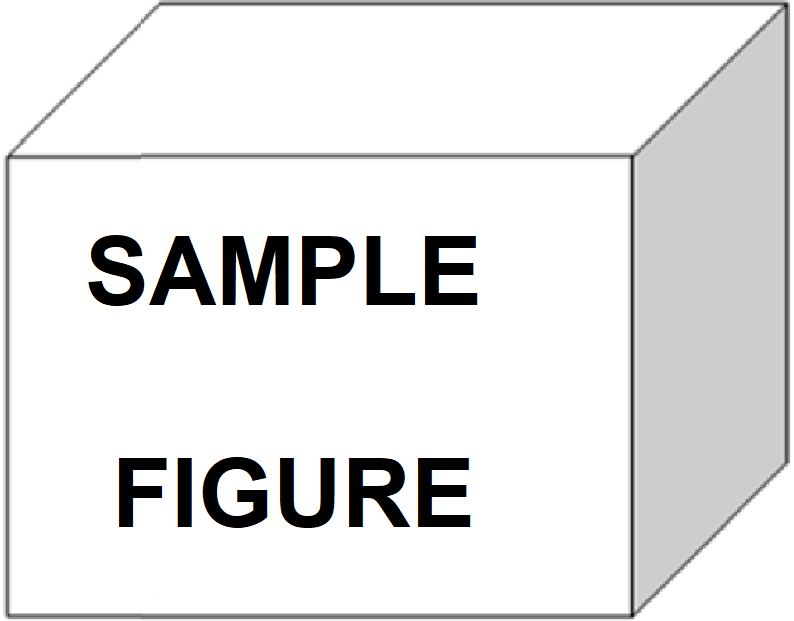
\includegraphics[width=10cm,keepaspectratio=true]{sekil1}
 % sekil1.eps: 0x0 pixel, 300dpi, 0.00x0.00 cm, bb=14 14 592 479
 \vspace*{4mm}
 \caption{Model structures.}
\end{figure}


\section{Hypothesis}

Lorem ipsum dolor sit amet, consectetur adipiscing elit. Praesent imperdiet, nisi 
nec aliquam cursus, dui turpis mollis nisl, ac consequat tellus sapien sit amet 
magna.

Lorem ipsum dolor sit amet, consectetur adipiscing elit. Praesent imperdiet, nisi 
nec aliquam cursus, dui turpis mollis nisl, ac consequat tellus sapien sit amet 
magna. Duis vel venenatis velit. Vestibulum ante ipsum primis in faucibus orci 
luctus et ultrices posuere cubilia Curae; Proin malesuada risus nec metus dapibus 
eu tincidunt lectus dignissim. 

Lorem ipsum dolor sit amet, consectetur adipiscing elit. Praesent imperdiet, nisi 
nec aliquam cursus, dui turpis mollis nisl, ac consequat tellus sapien sit amet 
magna. Duis vel venenatis velit. Vestibulum ante ipsum primis in faucibus orci 
luctus et ultrices posuere cubilia Curae; Proin malesuada risus nec metus dapibus 
eu tincidunt lectus dignissim. 

Lorem ipsum dolor sit amet, consectetur adipiscing elit \cite{harper2007}. Praesent imperdiet, nisi 
nec aliquam cursus, dui turpis mollis nisl, ac consequat tellus sapien sit amet 
magna. Duis vel venenatis velit. Vestibulum ante ipsum primis in faucibus orci 
luctus et ultrices posuere cubilia Curae; Proin malesuada risus nec metus dapibus 
eu tincidunt lectus dignissim \cite{unesco}.

Lorem ipsum dolor sit amet, consectetur adipiscing elit. Praesent imperdiet, nisi 
nec aliquam cursus, dui turpis mollis nisl, ac consequat tellus sapien sit amet 
magna. Duis vel venenatis velit. Vestibulum ante ipsum primis in faucibus orci 
luctus et ultrices posuere cubilia Curae; Proin malesuada risus nec metus dapibus 
eu tincidunt lectus dignissim.Lorem ipsum dolor sit amet, consectetur adipiscing elit. 
Praesent imperdiet, nisi nec aliquam cursus, dui turpis mollis nisl, ac consequat 
tellus \cite{mccaffrey88, moore91, nelson88, sisaky, simpsondvd, startrek, TS-40561, url-1, url-2, vanden2001} 
%\cite{moore91} \cite{nelson88} \cite{sisaky} \cite{simpsondvd} \cite{startrek} \cite{TS-40561} \cite{url-1} \cite{url-2} \cite{vanden2001}.

Duis vel venenatis velit. Vestibulum ante ipsum primis in faucibus orci 
luctus et ultrices posuere cubilia Curae; Proin malesuada risus nec metus dapibus 
eu tincidunt lectus dignissim.

Lorem ipsum dolor sit amet, consectetur adipiscing elit. Praesent imperdiet, nisi 
nec aliquam cursus, dui turpis mollis nisl, ac consequat tellus sapien sit amet 
magna. Duis vel venenatis velit. Vestibulum ante ipsum primis in faucibus orci 
luctus et ultrices posuere cubilia Curae; Proin malesuada risus nec metus dapibus 
eu tincidunt lectus dignissim.

\begin{table*}
{\setlength{\tabcolsep}{14pt}
\caption{Table captions must be ended with a full stop.}
\begin{center}
\vspace{-6mm}
\begin{tabular}{cccc}
\hline\hline
Column A & Column B & Column C & Column D \\
\hline
Row A & Row A & Row A & Row A \\
Row B & Row B & Row B & Row B \\
Row C & Row C & Row C & Row C \\
\hline
\end{tabular}
\vspace{-6mm}
\end{center}
\label{sitable3}}
\end{table*}

Lorem ipsum dolor sit amet, consectetur adipiscing elit. Praesent imperdiet, nisi 
nec aliquam cursus, dui turpis mollis nisl, ac consequat tellus sapien sit amet 
magna. Duis vel venenatis velit. Vestibulum ante ipsum primis in faucibus orci 
luctus et ultrices posuere cubilia Curae; Proin malesuada risus nec metus dapibus 
eu tincidunt lectus dignissim \cite{nelson88}.



%%%%%%%%%%%%%%%%%%%%%%%%%%%%%%%%%%%%%%%%%%%%%%%%%%%%%%%%%%%%%%%%%
\chapter{INTEGRATED DATA}\label{CH2}
%%%%%%%%%%%%%%%%%%%%%%%%%%%%%%%%%%%%%%%%%%%%%%%%%%%%%%%%%%%%%%%%%

\section{Purpose}

Class aptent taciti sociosqu ad litora torquent per conubia nostra, per inceptos himenaeos. Maecenas mattis porta
aliquet. Phasellus elit tortor, convallis vel gravida et, sollicitudin non metus. Etiam vel faucibus tortor. Morbi
fringilla semper nisl, non eleifend ligula placerat ac. Sed auctor varius commodo. Etiam tempor blandit elementum. Sed
pellentesque dolor id eros laoreet facilisis. Nunc orci magna, suscipit cursus luctus eget, venenatis nec libero.
Praesent fermentum velit ut mauris rutrum dignissim.

Nunc at tellus vitae metus rutrum convallis. Donec sollicitudin gravida elementum. Ut laoreet orci turpis. Phasellus
lectus erat, ullamcorper et pretium sed, venenatis quis justo. Nullam elementum, dui vitae egestas mollis, orci lorem
ornare tortor, non tempor nulla odio a lectus. Aenean semper tincidunt nisi, tristique commodo justo mollis et. Ut in
scelerisque nisl. Pellentesque quis velit augue. Suspendisse varius urna id quam egestas nec lacinia sapien dignissim.
Vivamus scelerisque pharetra pharetra. Cras tortor sem, rutrum ac interdum et, cursus ut libero. Praesent volutpat nisl
vel dui faucibus interdum vel vitae lectus. Morbi venenatis rutrum elit sit amet faucibus. Vestibulum lacinia nulla
fringilla mi molestie tempus. In interdum dolor sit amet mi aliquam commodo. Aliquam erat volutpat. Nullam nisi erat,
vestibulum sit amet molestie sit amet, accumsan quis dolor. 

\section{Internet Service Networks}

Curabitur sit amet quam quam, vitae accumsan arcu. Sed feugiat, risus non fringilla commodo, nisl eros fringilla ante,
nec imperdiet enim justo sit amet diam. Etiam mollis vulputate urna, ut scelerisque neque consequat in. Phasellus
luctus, turpis vel fermentum iaculis, felis nunc lacinia orci, sit amet rutrum nisi tellus eu risus. Mauris interdum
tristique risus vel varius. Donec rutrum tincidunt lacinia. Vestibulum pretium viverra consequat. Nullam at interdum
tellus. Aliquam tincidunt nulla vel massa lobortis sed aliquet orci elementum. Nullam non velit massa. Vivamus cursus
consectetur suscipit. Duis eros purus, vehicula ac ullamcorper non, imperdiet eu dolor. Integer nec velit nisl
\cite{moore91}. 

\begin{figure}
 \centering
 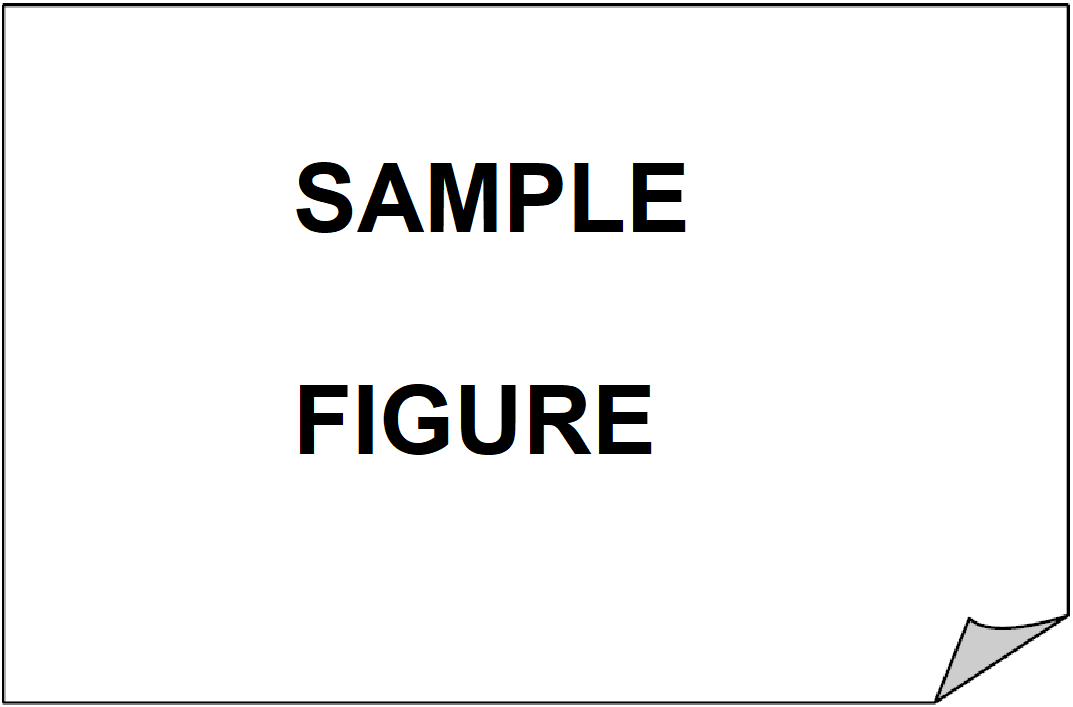
\includegraphics[width=10cm,keepaspectratio=true]{sekil2}
 \vspace*{4mm}
 \caption{Advanced Structures.}
 \label{fig:ch2-1}
\end{figure}

Lorem ipsum dolor sit amet, consectetur adipiscing elit. Sed ac augue vel dui 
adipiscing placerat et nec metus. Donec bibendum sodales mollis. Cras in lacus 
justo, at vestibulum quam. Sed semper, est sit amet consectetur ornare, leo est 
lacinia velit, adipiscing elementum lectus felis at sem. Aenean hendrerit erat eu 
lacus malesuada at sodales arcu egestas. Maecenas euismod urna ut sem luctus et 
congue metus vulputate. Ut pellentesque, neque eget fringilla elementum, ligula 
massa aliquet lorem, et varius nisi lacus vel diam. Etiam vitae metus sed orci 
rutrum fringilla. Phasellus sed velit quam. Mauris vestibulum, mauris a cursus 
adipiscing, nulla est hendrerit justo, ut fringilla eros velit ut mauris 
\cite{Wegener2000629}.

Sed et est vestibulum felis sagittis congue. Phasellus fringilla sem eu purus 
posuere ut viverra massa dignissim. Maecenas ornare neque velit. Vivamus interdum 
euismod elementum. Ut sit amet luctus ligula. Vivamus porttitor venenatis sem nec 
congue. Quisque sed lectus et nibh imperdiet vestibulum. Vivamus vel turpis leo. 
Proin suscipit iaculis nibh, nec dictum augue aliquet in. Praesent fermentum sem 
tempus orci molestie at facilisis dui sagittis. Etiam sit amet imperdiet sapien. 

\newpage
\section{Network Based Project Development}

Lorem ipsum dolor sit amet, consectetur adipiscing elit. Sed ac augue vel dui 
adipiscing placerat et nec metus. Donec bibendum sodales mollis. Cras in lacus 
justo, at vestibulum quam. Sed semper, est sit amet consectetur ornare, leo est 
lacinia velit, adipiscing elementum lectus felis at sem. Aenean hendrerit erat eu 
lacus malesuada at sodales arcu egestas. Maecenas euismod urna ut sem luctus et 
congue metus vulputate. Ut pellentesque, neque eget fringilla elementum, ligula 
massa aliquet lorem, et varius nisi lacus vel diam. Etiam vitae metus sed orci 
rutrum fringilla. Phasellus sed velit quam. Mauris vestibulum, mauris a cursus 
adipiscing, nulla est hendrerit justo, ut fringilla eros velit ut mauris.

Sed et est vestibulum felis sagittis congue. Phasellus fringilla sem eu purus 
posuere ut viverra massa dignissim. Maecenas ornare neque velit. Vivamus interdum 
euismod elementum. Ut sit amet luctus ligula. Vivamus porttitor venenatis sem nec 
congue. Quisque sed lectus et nibh imperdiet vestibulum. Vivamus vel turpis leo. 
Proin suscipit iaculis nibh, nec dictum augue aliquet in. Praesent fermentum sem 
tempus orci molestie at facilisis dui sagittis. Etiam sit amet imperdiet sapien. 
Donec convallis, quam in vestibulum cursus, nisl mi egestas felis, et porttitor 
ante ipsum quis turpis. Etiam ligula leo, sodales eget mollis eget, scelerisque 
vitae leo. Cum sociis natoque penatibus et magnis dis parturient montes, nascetur 
ridiculus mus. 

Lorem ipsum dolor sit amet, consectetur adipiscing elit. Sed ac augue vel dui 
adipiscing placerat et nec metus. Donec bibendum sodales mollis. Cras in lacus 
justo, at vestibulum quam. Sed semper, est sit amet consectetur ornare, leo est 
lacinia velit, adipiscing elementum lectus felis at sem. Aenean hendrerit erat eu 
lacus malesuada at sodales arcu egestas. Maecenas euismod urna ut sem luctus et 
congue metus vulputate. Ut pellentesque, neque eget fringilla elementum, ligula 
massa aliquet lorem, et varius nisi lacus vel diam. Etiam vitae metus sed orci 
rutrum fringilla. Phasellus sed velit quam. Mauris vestibulum, mauris a cursus 
adipiscing, nulla est hendrerit justo, ut fringilla eros velit ut mauris.

\begin{table*}
{\setlength{\tabcolsep}{14pt}
\caption{Table captions must be ended with a full stop.}
\begin{center}
\vspace{-6mm}
\begin{tabular}{cccc}
\hline\hline
Column A & Column B & Column C & Column D \\
\hline
Row A & Row A & Row A & Row A \\
Row B & Row B & Row B & Row B \\
Row C & Row C & Row C & Row C \\
\hline
\end{tabular}
\vspace{-6mm}
\end{center}
\label{tableforCh2.3}}
\end{table*}

Sed et est vestibulum felis sagittis congue. Phasellus fringilla sem eu purus 
posuere ut viverra massa dignissim. Maecenas ornare neque velit. Vivamus interdum 
euismod elementum. Ut sit amet luctus ligula. Vivamus porttitor venenatis sem nec 
congue. Quisque sed lectus et nibh imperdiet vestibulum. Vivamus vel turpis leo. 
Proin suscipit iaculis nibh, nec dictum augue aliquet in. Praesent fermentum sem 
tempus orci molestie at facilisis dui sagittis. Etiam sit amet imperdiet sapien. 
Donec convallis, quam in vestibulum cursus, nisl mi egestas felis, et porttitor 
ante ipsum quis turpis. Etiam ligula leo, sodales eget mollis eget, scelerisque 
vitae leo. Cum sociis natoque penatibus et magnis dis parturient montes, nascetur 
ridiculus mus \cite{Zuckerman199486}. 

%%%%%%%%%%%%%%%%%%%%%%%%%%%%%%%%%%%%%%%%%%%%%%%%%%%%%%%%%%%%%%%%%
\chapter{FLOW PREDICTION}\label{ch:fp}
%%%%%%%%%%%%%%%%%%%%%%%%%%%%%%%%%%%%%%%%%%%%%%%%%%%%%%%%%%%%%%%%%

\vspace{-12pt} %iki başlık alt alta. iki katı boşluk olmasın

\section{Purpose}

Lorem ipsum dolor sit amet, consectetur adipiscing elit. Sed ac augue vel dui 
adipiscing placerat et nec metus. Donec bibendum sodales mollis. Cras in lacus 
justo, at vestibulum quam. Sed semper, est sit amet consectetur ornare, leo est 
lacinia velit, adipiscing elementum lectus felis at sem. Aenean hendrerit erat eu 
lacus malesuada at sodales arcu egestas. Maecenas euismod urna ut sem luctus et 
congue metus vulputate. Ut pellentesque, neque eget fringilla elementum, ligula 
massa aliquet lorem, et varius nisi lacus vel diam. Etiam vitae metus sed orci 
rutrum fringilla. Phasellus sed velit quam. Mauris vestibulum, mauris a cursus 
adipiscing, nulla est hendrerit justo, ut fringilla eros velit ut mauris.

Sed et est vestibulum felis sagittis congue. Phasellus fringilla sem eu purus 
posuere ut viverra massa dignissim. Maecenas ornare neque velit. Vivamus interdum 
euismod elementum. Ut sit amet luctus ligula. Vivamus porttitor venenatis sem nec 
congue. Quisque sed lectus et nibh imperdiet vestibulum. Vivamus vel turpis leo. 
Proin suscipit iaculis nibh, nec dictum augue aliquet in. Praesent fermentum sem 
tempus orci molestie at facilisis dui sagittis. Etiam sit amet imperdiet sapien. 

\subsection{Artificial neural networks}

Lorem ipsum dolor sit amet, consectetur adipiscing elit. Sed ac augue vel dui 
adipiscing placerat et nec metus. Donec bibendum sodales mollis. Cras in lacus 
justo, at vestibulum quam. Sed semper, est sit amet consectetur ornare, leo est 
lacinia velit, adipiscing elementum lectus felis at sem. Aenean hendrerit erat eu 
lacus malesuada at sodales arcu egestas. Maecenas euismod urna ut sem luctus et 
congue metus vulputate.

\begin{figure}
 \centering
 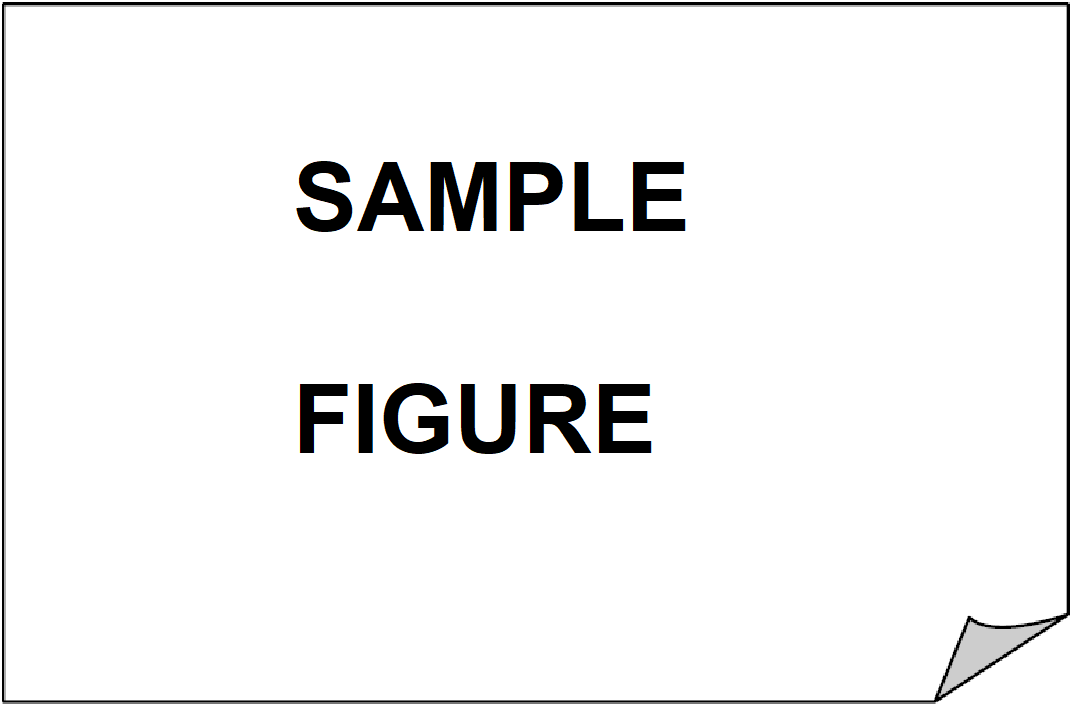
\includegraphics[width=230pt,keepaspectratio=true]{sekil3}
 \vspace*{4mm}
 \caption[Short version for LoF]{Long version to appear next to the figure.}
 \label{fig:3-1-1}
\end{figure}

Lorem ipsum dolor sit amet, consectetur adipiscing elit. Sed ac augue vel dui 
adipiscing placerat et nec metus. Donec bibendum sodales mollis. Cras in lacus 
justo, at vestibulum quam. Sed semper, est sit amet consectetur ornare, leo est 
lacinia velit, adipiscing elementum lectus felis at sem. Aenean hendrerit erat eu 
lacus malesuada at sodales arcu egestas. Maecenas euismod urna ut sem luctus et 
congue metus vulputate. Ut pellentesque, neque eget fringilla elementum, ligula 
massa aliquet lorem, et varius nisi lacus vel diam. Etiam vitae metus sed orci 
rutrum fringilla. Phasellus sed velit quam. Mauris vestibulum, mauris a cursus 
adipiscing, nulla est hendrerit justo, ut fringilla eros velit ut mauris.

Sed et est vestibulum felis sagittis congue. Phasellus fringilla sem eu purus 
posuere ut viverra massa dignissim. Maecenas ornare neque velit. Vivamus interdum 
euismod elementum. Ut sit amet luctus ligula. Vivamus porttitor venenatis sem nec 
congue. Quisque sed lectus et nibh imperdiet vestibulum. Vivamus vel turpis leo. 
Proin suscipit iaculis nibh, nec dictum augue aliquet in. Praesent fermentum sem 
tempus orci molestie at facilisis dui sagittis. Etiam sit amet imperdiet sapien.

\subsection{Autoregressive models}

Lorem ipsum dolor sit amet, consectetur adipiscing elit. Sed ac augue vel dui 
adipiscing placerat et nec metus. Donec bibendum sodales mollis. Cras in lacus 
justo, at vestibulum quam. Sed semper, est sit amet consectetur ornare, leo est 
lacinia velit, adipiscing elementum lectus felis at sem. Aenean hendrerit erat eu 
lacus malesuada at sodales arcu egestas. 

\begin{equation}
\label{eq:3-1}
   y_{t}  \equiv \phi_{1} y_{t-1} + \epsilon_{t}
\end{equation}

Maecenas euismod urna ut sem luctus et (\ref{eq:3-1})
congue metus vulputate. Ut pellentesque, neque eget fringilla elementum, ligula 
massa aliquet lorem, et varius nisi lacus vel diam. Etiam vitae metus sed orci 
rutrum fringilla. Phasellus sed velit quam. Mauris vestibulum, mauris a cursus 
adipiscing, nulla est hendrerit justo, ut fringilla eros velit ut mauris.

\subsection{Process based model: SWAT}

Lorem ipsum dolor sit amet, consectetur adipiscing elit. Sed ac augue vel dui 
adipiscing placerat et nec metus. Donec bibendum sodales mollis. Cras in lacus 
justo, at vestibulum quam. Sed semper, est sit amet consectetur ornare, leo est 
lacinia velit, adipiscing elementum lectus felis at sem. Aenean hendrerit erat eu 
lacus malesuada at sodales arcu egestas. Maecenas euismod urna ut sem luctus et 
congue metus vulputate. Ut pellentesque, neque eget fringilla elementum, ligula 
massa aliquet lorem, et varius nisi lacus vel diam. Etiam vitae metus sed orci 
rutrum fringilla. Phasellus sed velit quam. Mauris vestibulum, mauris a cursus 
adipiscing, nulla est hendrerit justo, ut fringilla eros velit ut mauris.

Sed et est vestibulum felis sagittis congue. Phasellus fringilla sem eu purus 
posuere ut viverra massa dignissim. Maecenas ornare neque velit. Vivamus interdum 
euismod elementum. Ut sit amet luctus ligula. Vivamus porttitor venenatis sem nec 
congue. Quisque sed lectus et nibh imperdiet vestibulum. Vivamus vel turpis leo. 
Proin suscipit iaculis nibh, nec dictum augue aliquet in. Praesent fermentum sem 
tempus orci molestie at facilisis dui sagittis. Etiam sit amet imperdiet sapien.

\begin{figure}[h!]
 \centering
 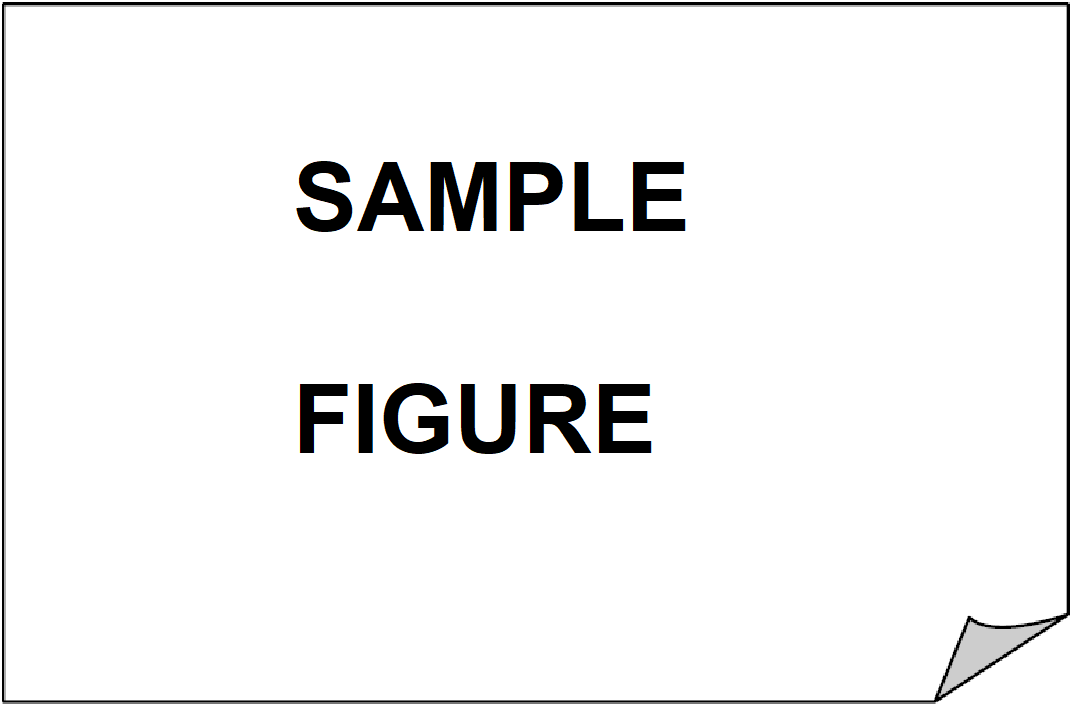
\includegraphics[width=230pt,keepaspectratio=true]{sekil3}
 \vspace{4mm}
 \caption{For a multi-line figure captions, it is important that all the
  lines of the caption are aligned.}
 \label{fig:3-1-3}
\end{figure}

Lorem ipsum dolor sit amet, consectetur adipiscing elit. Sed ac augue vel dui 
adipiscing placerat et nec metus. Donec bibendum sodales mollis. Cras in lacus 
justo, at vestibulum quam. Sed semper, est sit amet consectetur ornare, leo est 
lacinia velit, adipiscing elementum lectus felis at sem. Aenean hendrerit erat eu 
lacus malesuada at sodales arcu egestas. Maecenas euismod urna ut sem luctus et 
congue metus vulputate. Ut pellentesque, neque eget fringilla elementum, ligula 
massa aliquet lorem, et varius nisi lacus vel diam. Etiam vitae metus sed orci 
rutrum fringilla. Phasellus sed velit quam. Mauris vestibulum, mauris a cursus 
adipiscing, nulla est hendrerit justo, ut fringilla eros velit ut mauris.

Sed et est vestibulum felis sagittis congue. Phasellus fringilla sem eu purus 
posuere ut viverra massa dignissim. Maecenas ornare neque velit. Vivamus interdum 
euismod elementum. Ut sit amet luctus ligula. Vivamus porttitor venenatis sem nec 
congue. Quisque sed lectus et nibh imperdiet vestibulum. Vivamus vel turpis leo. 
Proin suscipit iaculis nibh, nec dictum augue aliquet in. Praesent fermentum sem 
tempus orci molestie at facilisis dui sagittis. Etiam sit amet imperdiet sapien.

\subsection{Multi variable analysis}

Lorem ipsum dolor sit amet, consectetur adipiscing elit. Sed ac augue vel dui 
adipiscing placerat et nec metus. Donec bibendum sodales mollis. Cras in lacus 
justo, at vestibulum quam. Sed semper, est sit amet consectetur ornare, leo est 
lacinia velit, adipiscing elementum lectus felis at sem. Aenean hendrerit erat eu 
lacus malesuada at sodales arcu egestas. Maecenas euismod urna ut sem luctus et 
congue metus vulputate. Ut pellentesque, neque eget fringilla elementum, ligula 
massa aliquet lorem, et varius nisi lacus vel diam. Etiam vitae metus sed orci 
rutrum fringilla. Phasellus sed velit quam. Mauris vestibulum, mauris a cursus 
adipiscing, nulla est hendrerit justo, ut fringilla eros velit ut mauris.

Sed et est vestibulum felis sagittis congue. Phasellus fringilla sem eu purus 
posuere ut viverra massa dignissim. Maecenas ornare neque velit. Vivamus interdum 
euismod elementum. Ut sit amet luctus ligula. Vivamus porttitor venenatis sem nec 
congue. Quisque sed lectus et nibh imperdiet vestibulum. Vivamus vel turpis leo. 
Proin suscipit iaculis nibh, nec dictum augue aliquet in. Praesent fermentum sem 
tempus orci molestie at facilisis dui sagittis. Etiam sit amet imperdiet sapien.

\begin{figure}
 \centering
 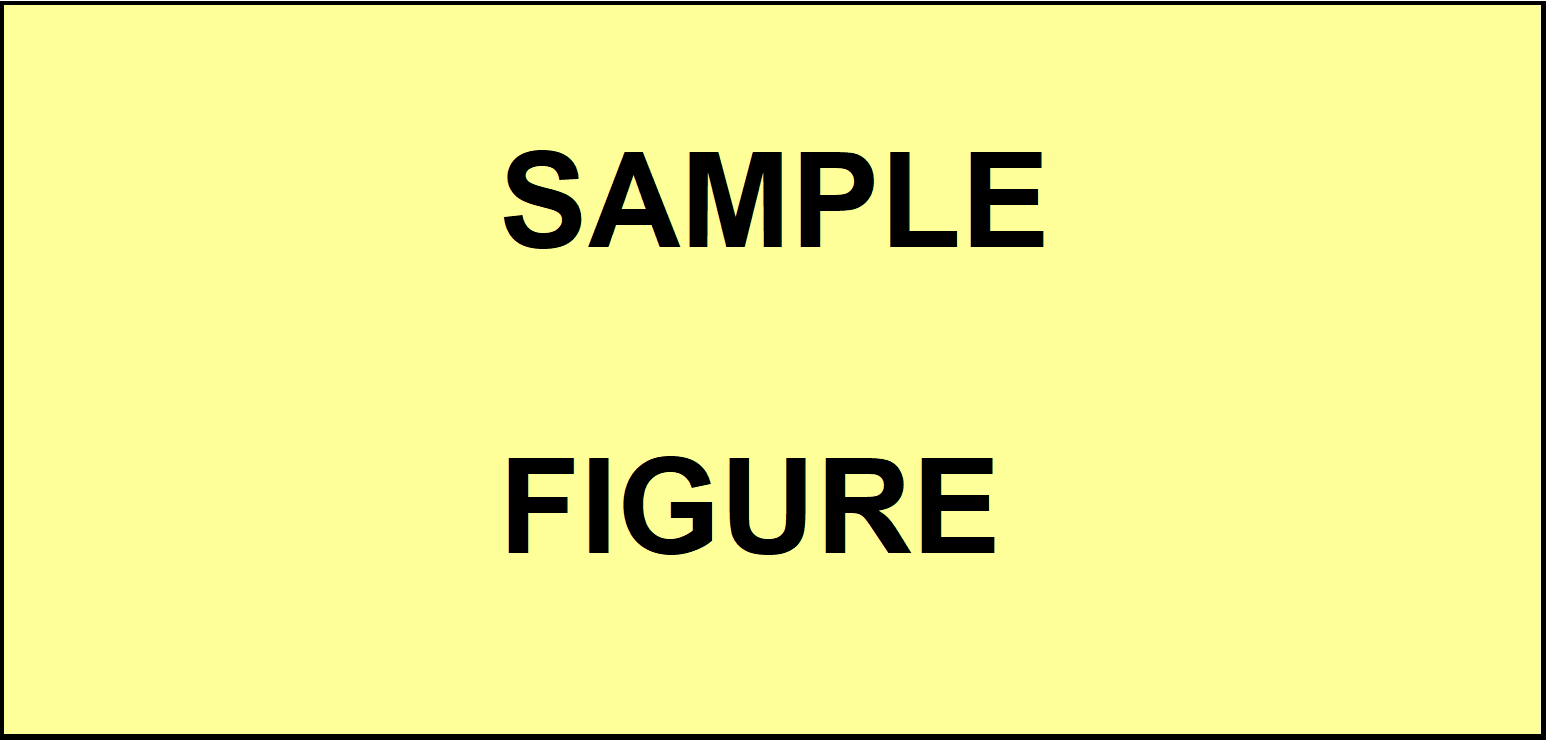
\includegraphics[width=290pt,keepaspectratio=true]{sekil4}
 % sekil4.eps: 0x0 pixel, 300dpi, 0.00x0.00 cm, bb=14 14 1148 603
 \vspace{4mm}
 \caption{Figure captions must be ended with a full stop.}
 \label{fig:3-1-4}
\end{figure}

Lorem ipsum dolor sit amet, consectetur adipiscing elit. Sed ac augue vel dui 
adipiscing placerat et nec metus. Donec bibendum sodales mollis. Cras in lacus 
justo, at vestibulum quam. Sed semper, est sit amet consectetur ornare, leo est 
lacinia velit, adipiscing elementum lectus felis at sem. Aenean hendrerit erat eu 
lacus malesuada at sodales arcu egestas. Maecenas euismod urna ut sem luctus et 
congue metus vulputate. Ut pellentesque, neque eget fringilla elementum, ligula 
massa aliquet lorem, et varius nisi lacus vel diam. Etiam vitae metus sed orci 
rutrum fringilla. Phasellus sed velit quam. Mauris vestibulum, mauris a cursus 
adipiscing, nulla est hendrerit justo, ut fringilla eros velit ut mauris.
\begin{equation}
    D\left(C_{A},C_{B}\right) = \min X_{A}\in C_{A},X_{B}\in C_{B} 
     d\left(X_{A},X_{B}\right)  
\end{equation}
Sed et est vestibulum felis sagittis congue. Phasellus fringilla sem eu purus 
posuere ut viverra massa dignissim. Maecenas ornare neque velit. Vivamus interdum 
euismod elementum. Ut sit amet luctus ligula. Vivamus porttitor venenatis sem nec 
congue. Quisque sed lectus et nibh imperdiet vestibulum. Vivamus vel turpis leo. 
Proin suscipit iaculis nibh, nec dictum augue aliquet in. Praesent fermentum sem 
tempus orci molestie at facilisis dui sagittis. Etiam sit amet imperdiet sapien.

\begin{landscape}
\thispagestyle{empty}
 \begin{figure}
 \vspace{-2mm}
 \centering
 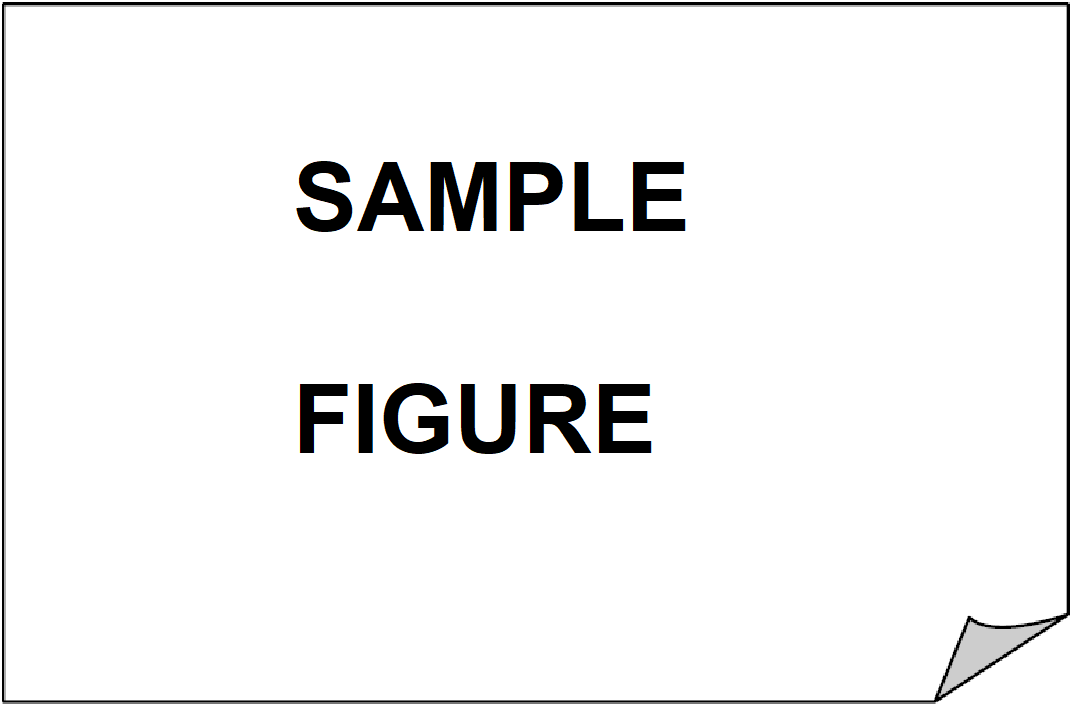
\includegraphics[width=450pt,keepaspectratio=true]{sekil3}
 % sekil3.eps: 0x0 pixel, 300dpi, 0.00x0.00 cm, bb=14 14 1155 740
 \vspace{4mm}
 \caption{Landscape-oriented, full-page figure.}    
      \vspace{55mm}
      \hspace{0cm}\pageref{fig:cshapeMapVMAT}
      \label{fig:cshapeMapVMAT}
\end{figure}
\end{landscape}

\section{Practical Applications}

Lorem ipsum dolor sit amet, consectetur adipiscing elit. Sed ac augue vel dui 
adipiscing placerat et nec metus. Donec bibendum sodales mollis. Cras in lacus 
justo, at vestibulum quam. Sed semper, est sit amet consectetur ornare, leo est 
lacinia velit, adipiscing elementum lectus felis at sem. Aenean hendrerit erat eu 
lacus malesuada at sodales arcu egestas. Maecenas euismod urna ut sem luctus et 
congue metus vulputate. Ut pellentesque, neque eget fringilla elementum, ligula 
massa aliquet lorem, et varius nisi lacus vel diam. Etiam vitae metus sed orci 
rutrum fringilla. Phasellus sed velit quam. Mauris vestibulum, mauris a cursus 
adipiscing, nulla est hendrerit justo, ut fringilla eros velit ut mauris.

Lorem ipsum dolor sit amet, consectetur adipiscing elit. Sed ac augue vel dui 
adipiscing placerat et nec metus. Donec bibendum sodales mollis. Cras in lacus 
justo, at vestibulum quam. Sed semper, est sit amet consectetur ornare, leo est 
lacinia velit, adipiscing elementum lectus felis at sem. Aenean hendrerit erat eu 
lacus malesuada at sodales arcu egestas. Maecenas euismod urna ut sem luctus et 
congue metus vulputate. Ut pellentesque, neque eget fringilla elementum, ligula 
massa aliquet lorem, et varius nisi lacus vel diam.

\section{Application Data}

Lorem ipsum dolor sit amet, consectetur adipiscing elit. Sed ac augue vel dui 
adipiscing placerat et nec metus. Donec bibendum sodales mollis. Cras in lacus 
justo, at vestibulum quam. Sed semper, est sit amet consectetur ornare, leo est 
lacinia velit, adipiscing elementum lectus felis at sem. Aenean hendrerit erat eu 
lacus malesuada at sodales arcu egestas. Maecenas euismod urna ut sem luctus et 
congue metus vulputate. Ut pellentesque, neque eget fringilla elementum, ligula 
massa aliquet lorem, et varius nisi lacus vel diam. Etiam vitae metus sed orci 
rutrum fringilla. Phasellus sed velit quam. Mauris vestibulum, mauris a cursus 
adipiscing, nulla est hendrerit justo, ut fringilla eros velit ut mauris.

Lorem ipsum dolor sit amet, consectetur adipiscing elit. Sed ac augue vel dui 
adipiscing placerat et nec metus. Donec bibendum sodales mollis. Cras in lacus 
justo, at vestibulum quam. Sed semper, est sit amet consectetur ornare, leo est 
lacinia velit, adipiscing elementum lectus felis at sem. Aenean hendrerit erat eu 
lacus malesuada at sodales arcu egestas. Maecenas euismod urna ut sem luctus et 
congue metus vulputate. Ut pellentesque, neque eget fringilla elementum, ligula 
massa aliquet lorem, et varius nisi lacus vel diam. Etiam vitae metus sed orci 
rutrum fringilla. Phasellus sed velit quam. Mauris vestibulum, mauris a cursus 
adipiscing, nulla est hendrerit justo, ut fringilla eros velit ut mauris
\cite{Wegener2000629}.

% ---------------------------------------------------------------- %
% Numbered citation.						   %
% ---------------------------------------------------------------- %

Lorem ipsum dolor sit amet, consectetur adipiscing elit. Sed ac augue vel dui 
adipiscing placerat et nec metus \cite{Wolchik2000843}. 
Donec bibendum sodales mollis. Cras in lacus 
justo, at vestibulum quam. Sed semper, est sit amet consectetur ornare, leo est 
lacinia velit, adipiscing elementum lectus felis at sem. Aenean hendrerit erat eu 
lacus malesuada at sodales arcu egestas. Maecenas euismod urna ut sem luctus et 
congue metus vulputate. Ut pellentesque, neque eget fringilla elementum, ligula 
massa aliquet lorem, et varius nisi lacus vel diam. Etiam vitae metus sed orci 
rutrum fringilla. Phasellus sed velit quam \cite{Zuckerman199486}. 
Mauris vestibulum, mauris a cursus 
adipiscing, nulla est hendrerit justo, ut fringilla eros velit ut mauris.

% ---------------------------------------------------------------- %
% Page numbers must be on the bottom-middle of short side (when    %
% portrait-oriented), or bottom-middle of long side (when	   %
% landscape-oriented)						   %
% ---------------------------------------------------------------- %

\begin{landscape}
\thispagestyle{empty}
 
\begin{table*}
\vspace{-3mm}
{\setlength{\tabcolsep}{14pt}
\caption{Prof. Dr. Galip TEPEHAN  \,\,\, Captioning in landscape-oriented pages:
the most important aspect is to align the lines horizontally.}
\begin{center}
\vspace{-6mm}
\begin{tabular}{lccrrrrr}
\hline\hline
\multirow{2}{*}{Parametre} & \multirow{2}{*}{Column 2} & \multirow{2}{*}{Column 3} & \multicolumn{3}{c|}{Column 4} & \multicolumn{2}{c}{Column 5}\\ \cline{4-8}
  & & & Subcolumn & Subcolumn & Subcolumn & Subcolumn & Subcolumn\\
\hline
Row 1 & -7.680442 & 7.6986348 & 0.00 & 0.00 & 0.00 & 12 & 12 \\
Row 2 & 140 & - & 0.50 & 0.00 & 0.00 & 0 & 0 \\
Row 3 & 37.174357 & 37.16192697 & 0.00 & 0.00 & 0.00 & 0 & 24 \\
Row 4 & 140 & - & 0.50 & 0.00 & 0.00 & 0 & 0 \\
Row 5 & 37.174357 & 37.16192697 & 0.00 & 0.00 & 0.00 & 0 & 24 \\
Row 6 & 140 & - & 0.50 & 0.00 & 0.00 & 0 & 0 \\
Row 7 & 37.174357 & 37.16192697 & 0.00 & 0.00 & 0.00 & 0 & 24 \\
Row 8 & 140 & - & 0.50 & 0.00 & 0.00 & 0 & 0 \\
Row 9 & 37.174357 & 37.16192697 & 0.00 & 0.00 & 0.00 & 0 & 24 \\
Row 10 & 140 & - & 0.50 & 0.00 & 0.00 & 0 & 0 \\
Row 11 & 37.174357 & 37.16192697 & 0.00 & 0.00 & 0.00 & 0 & 24 \\
Row 12 & 140 & - & 0.50 & 0.00 & 0.00 & 0 & 0 \\
Row 13 & 37.174357 & 37.16192697 & 0.00 & 0.00 & 0.00 & 0 & 24 \\
Row 14 & 140 & - & 0.50 & 0.00 & 0.00 & 0 & 0 \\
Row 15 & 37.174357 & 37.16192697 & 0.00 & 0.00 & 0.00 & 0 & 24 \\
\end{tabular}
\end{center}
\begin{center}
      \vspace{53mm}
      \hspace{0cm}\pageref{table:galip}
      \label{table:galip}
\end{center}
}
\end{table*}

\end{landscape}
%%%%%%%%%%%%%%%%%%%%%%%%%%%%%%%%%%%%%%%%%%%%%%%%%%%%%%%%%%%%%%%%%
\chapter{(IF NECESSARY) CHAPTER 4}\label{ch:ifnecch4}
%%%%%%%%%%%%%%%%%%%%%%%%%%%%%%%%%%%%%%%%%%%%%%%%%%%%%%%%%%%%%%%%%

Lorem ipsum dolor sit amet, consectetur adipiscing elit. Sed ac augue vel dui 
adipiscing placerat et nec metus. Donec bibendum sodales mollis. Cras in lacus 
justo, at vestibulum quam. Sed semper, est sit amet consectetur ornare, leo est 
lacinia velit, adipiscing elementum lectus felis at sem. Aenean hendrerit erat eu 
lacus malesuada at sodales arcu egestas. Maecenas euismod urna ut sem luctus et 
congue metus vulputate. Ut pellentesque, neque eget fringilla elementum, ligula 
massa aliquet lorem, et varius nisi lacus vel diam. Etiam vitae metus sed orci 
rutrum fringilla. Phasellus sed velit quam. Mauris vestibulum, mauris a cursus 
adipiscing, nulla est hendrerit justo, ut fringilla eros velit ut mauris.

\section{Practical Application of This Study}

Lorem ipsum dolor sit amet, consectetur adipiscing elit. Sed ac augue vel dui 
adipiscing placerat et nec metus. Donec bibendum sodales mollis. Cras in lacus 
justo, at vestibulum quam. Sed semper, est sit amet consectetur ornare, leo est 
lacinia velit, adipiscing elementum lectus felis at sem. Aenean hendrerit erat eu 
lacus malesuada at sodales arcu egestas. Maecenas euismod urna ut sem luctus et 
congue metus vulputate. Ut pellentesque, neque eget fringilla elementum, ligula 
massa aliquet lorem, et varius nisi lacus vel diam. Etiam vitae metus sed orci 
rutrum fringilla. Phasellus sed velit quam. Mauris vestibulum, mauris a cursus 
adipiscing, nulla est hendrerit justo, ut fringilla eros velit ut mauris.

\section{Second Level Title: First Letters Capital}

Lorem ipsum dolor sit amet, consectetur adipiscing elit. Sed ac augue vel dui 
adipiscing placerat et nec metus. Donec bibendum sodales mollis. Cras in lacus 
justo, at vestibulum quam. Sed semper, est sit amet consectetur ornare, leo est 
lacinia velit, adipiscing elementum lectus felis at sem. 

\subsection{Third level title: Only first letter capital}

Lorem ipsum dolor sit amet, consectetur adipiscing elit. Sed ac augue vel dui 
adipiscing placerat et nec metus. Donec bibendum sodales mollis. Cras in lacus 
justo, at vestibulum quam. Sed semper, est sit amet consectetur ornare, leo est 
lacinia velit, adipiscing elementum lectus felis at sem.

\subsubsection{Fourth level title: Only first letter capital}

Lorem ipsum dolor sit amet, consectetur adipiscing elit. Sed ac augue vel dui 
adipiscing placerat et nec metus. Donec bibendum sodales mollis. Cras in lacus 
justo, at vestibulum quam. Sed semper, est sit amet consectetur ornare, leo est 
lacinia velit, adipiscing elementum lectus felis at sem.

\subsubsubsection{Fifth level title: no numbering
after fourth level titles}

Lorem ipsum dolor sit amet, consectetur adipiscing elit. Sed ac augue vel dui 
adipiscing placerat et nec metus. Donec bibendum sodales mollis. Cras in lacus 
justo, at vestibulum quam. Sed semper, est sit amet consectetur ornare, leo est 
lacinia velit, adipiscing elementum lectus felis at sem.

\begin{figure}
 \centering
 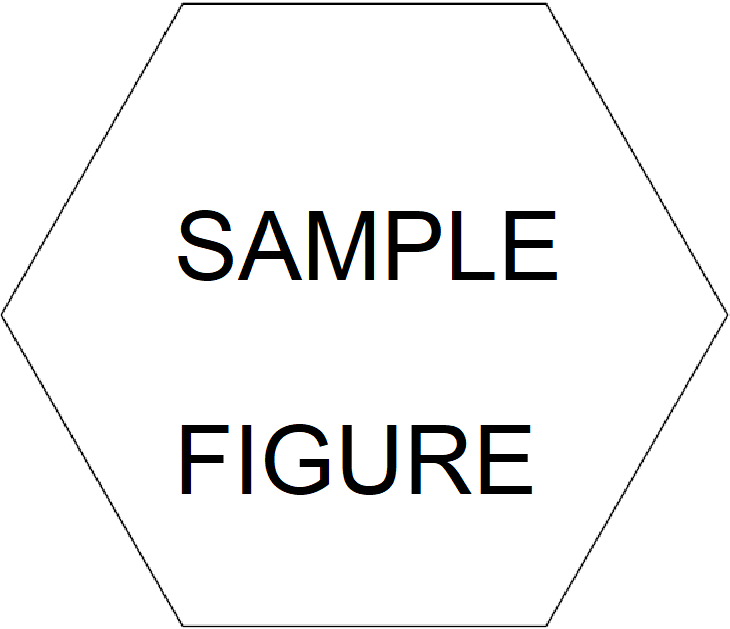
\includegraphics[width=230pt,keepaspectratio=true]{sekil6}
 % sekil6.eps: 0x0 pixel, 300dpi, 0.00x0.00 cm, bb=14 14 555 489
 \vspace{2mm}
 \caption{For a multi-line figure captions, it is important that all the
  lines of the caption are aligned.}
 \label{fig:4-1}
\end{figure}

Lorem ipsum dolor sit amet, consectetur adipiscing elit. Sed ac augue vel dui 
adipiscing placerat et nec metus. Donec bibendum sodales mollis. Cras in lacus 
justo, at vestibulum quam. Sed semper, est sit amet consectetur ornare, leo est 
lacinia velit, adipiscing elementum lectus felis at sem.

\begin{table*}
{\setlength{\tabcolsep}{14pt}
\caption{Example table.}
\begin{center}
\vspace{-6mm}
\begin{tabular}{cccc}
\hline\hline
Column A & Column B & Column C & Column D \\
\hline
Row A & Row A & Row A & Row A \\
Row B & Row B & Row B & Row B \\
Row C & Row C & Row C & Row C \\
\hline
\end{tabular}
\vspace{-6mm}
\end{center}
\label{tableforCh4-1}}
\end{table*}

Lorem ipsum dolor sit amet, consectetur adipiscing elit. Sed ac augue vel dui 
adipiscing placerat et nec metus. Donec bibendum sodales mollis. Cras in lacus 
justo, at vestibulum quam. Sed semper, est sit amet consectetur ornare, leo est 
lacinia velit, adipiscing elementum lectus felis at sem. Aenean hendrerit erat eu 
lacus malesuada at sodales arcu egestas. Maecenas euismod urna ut sem luctus et 
congue metus vulputate. Ut pellentesque, neque eget fringilla elementum, ligula 
massa aliquet lorem, et varius nisi lacus vel diam. Etiam vitae metus sed orci 
rutrum fringilla. Phasellus sed velit quam. Mauris vestibulum, mauris a cursus 
adipiscing, nulla est hendrerit justo, ut fringilla eros velit ut mauris.
%%%%%%%%%%%%%%%%%%%%%%%%%%%%%%%%%%%%%%%%%%%%%%%%%%%%%%%%%%%%%%%%%
\chapter{(IF NECESSARY) CHAPTER 5}\label{ch:ifnecch5}
%%%%%%%%%%%%%%%%%%%%%%%%%%%%%%%%%%%%%%%%%%%%%%%%%%%%%%%%%%%%%%%%%

Lorem ipsum dolor sit amet, consectetur adipiscing elit. Sed ac augue vel dui 
adipiscing placerat et nec metus. Donec bibendum sodales mollis. Cras in lacus 
justo, at vestibulum quam. Sed semper, est sit amet consectetur ornare, leo est 
lacinia velit, adipiscing elementum lectus felis at sem. Aenean hendrerit erat eu 
lacus malesuada at sodales arcu egestas. Maecenas euismod urna ut sem luctus et 
congue metus vulputate. Ut pellentesque, neque eget fringilla elementum, ligula 
massa aliquet lorem, et varius nisi lacus vel diam. Etiam vitae metus sed orci 
rutrum fringilla. Phasellus sed velit quam. Mauris vestibulum, mauris a cursus 
adipiscing, nulla est hendrerit justo, ut fringilla eros velit ut mauris.

\section{Practical Application of This Study}

Lorem ipsum dolor sit amet, consectetur adipiscing elit. Sed ac augue vel dui 
adipiscing placerat et nec metus. Donec bibendum sodales mollis. Cras in lacus 
justo, at vestibulum quam. Sed semper, est sit amet consectetur ornare, leo est 
lacinia velit, adipiscing elementum lectus felis at sem. Aenean hendrerit erat eu 
lacus malesuada at sodales arcu egestas. Maecenas euismod urna ut sem luctus et 
congue metus vulputate. Ut pellentesque, neque eget fringilla elementum, ligula 
massa aliquet lorem, et varius nisi lacus vel diam. Etiam vitae metus sed orci 
rutrum fringilla. Phasellus sed velit quam. Mauris vestibulum, mauris a cursus 
adipiscing, nulla est hendrerit justo, ut fringilla eros velit ut mauris.

\section{Second Level Title: First Letters Capital}

Lorem ipsum dolor sit amet, consectetur adipiscing elit. Sed ac augue vel dui 
adipiscing placerat et nec metus. Donec bibendum sodales mollis. Cras in lacus 
justo, at vestibulum quam. Sed semper, est sit amet consectetur ornare, leo est 
lacinia velit, adipiscing elementum lectus felis at sem. 

\subsection{Third level title: Only first letter capital}

Lorem ipsum dolor sit amet, consectetur adipiscing elit. Sed ac augue vel dui 
adipiscing placerat et nec metus. Donec bibendum sodales mollis. Cras in lacus 
justo, at vestibulum quam. Sed semper, est sit amet consectetur ornare, leo est 
lacinia velit, adipiscing elementum lectus felis at sem.

\subsubsection{Fourth level title: Only first letter capital}

Lorem ipsum dolor sit amet, consectetur adipiscing elit. Sed ac augue vel dui 
adipiscing placerat et nec metus. Donec bibendum sodales mollis. Cras in lacus 
justo, at vestibulum quam. Sed semper, est sit amet consectetur ornare, leo est 
lacinia velit, adipiscing elementum lectus felis at sem.

{\bf Fifth level title: No numbering after fourth level titles}

Lorem ipsum dolor sit amet, consectetur adipiscing elit. Sed ac augue vel dui 
adipiscing placerat et nec metus. Donec bibendum sodales mollis. Cras in lacus 
justo, at vestibulum quam. Sed semper, est sit amet consectetur ornare, leo est 
lacinia velit, adipiscing elementum lectus felis at sem.

\begin{figure}
 \centering
 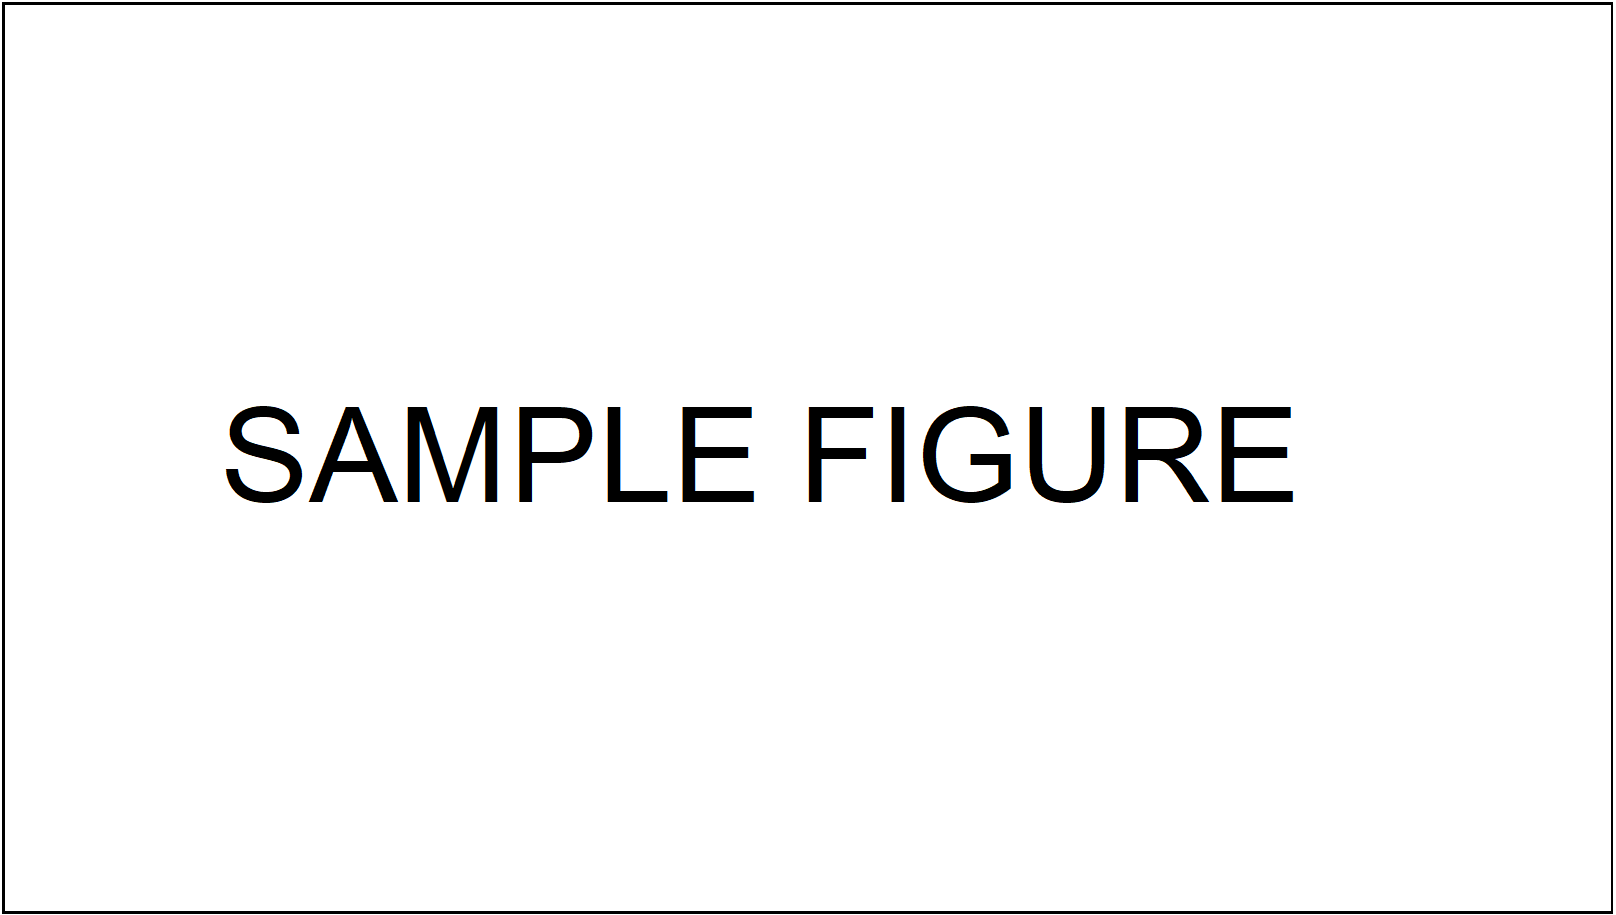
\includegraphics[width=230pt,keepaspectratio=true]{sekil5}
 % sekil5.eps: 0x0 pixel, 300dpi, 0.00x0.00 cm, bb=14 14 1193 701
 \vspace{4mm}
 \caption{For a multi-line figure captions, it is important that all the
  lines of the caption are aligned.}

 \label{fig:5-1}
\end{figure}

Lorem ipsum dolor sit amet, consectetur adipiscing elit. Sed ac augue vel dui 
adipiscing placerat et nec metus. Donec bibendum sodales mollis. Cras in lacus 
justo, at vestibulum quam. Sed semper, est sit amet consectetur ornare, leo est 
lacinia velit, adipiscing elementum lectus felis at sem.

\begin{table*}
{\setlength{\tabcolsep}{14pt}
\caption{Example table in chapter 5.}
\begin{center}
\vspace{-6mm}
\begin{tabular}{cccc}
\hline\hline
Column A & Column B & Column C & Column D \\
\hline
Row A & Row A & Row A & Row A \\
Row B & Row B & Row B & Row B \\
Row C & Row C & Row C & Row C \\
\hline
\end{tabular}
\vspace{-6mm}
\end{center}
\label{tableforCh5-1}}
\end{table*}

Lorem ipsum dolor sit amet, consectetur adipiscing elit. Sed ac augue vel dui 
adipiscing placerat et nec metus. Donec bibendum sodales mollis. Cras in lacus 
justo, at vestibulum quam. Sed semper, est sit amet consectetur ornare, leo est 
lacinia velit, adipiscing elementum lectus felis at sem. Aenean hendrerit erat eu 
lacus malesuada at sodales arcu egestas. Maecenas euismod urna ut sem luctus et 
congue metus vulputate. Ut pellentesque, neque eget fringilla elementum, ligula 
massa aliquet lorem, et varius nisi lacus vel diam. Etiam vitae metus sed orci 
rutrum fringilla. Phasellus sed velit quam. Mauris vestibulum, mauris a cursus 
adipiscing, nulla est hendrerit justo, ut fringilla eros velit ut mauris.
%%%%%%%%%%%%%%%%%%%%%%%%%%%%%%%%%%%%%%%%%%%%%%%%%%%%%%%%%%%%%%%%%
\chapter{CONCLUSIONS}\label{ch:ch6}
%%%%%%%%%%%%%%%%%%%%%%%%%%%%%%%%%%%%%%%%%%%%%%%%%%%%%%%%%%%%%%%%%

Lorem ipsum dolor sit amet, consectetur adipiscing elit. Sed ac augue vel dui 
a\-di\-pi\-scing pla\-ce\-rat et nec me\-tus. Donec bibendum sodales mollis. Cras in lacus 
justo, at vestibulum quam. Sed semper, est sit amet consectetur ornare, leo est 
lacinia velit, adipiscing elementum lectus felis at sem. Aenean hendrerit erat eu 
lacus malesuada at sodales arcu egestas. Maecenas euismod urna ut sem luctus et 
congue metus vulputate. Ut pellentesque, neque eget fringilla elementum, ligula 
massa aliquet lorem, et varius nisi lacus vel diam. Etiam vitae metus sed orci 
rutrum fringilla. Phasellus sed velit quam. Mauris vestibulum, mauris a cursus 
adipiscing, nulla est hendrerit justo, ut fringilla eros velit ut mauris.

\section{Practical Application of This Study}

Lorem ipsum dolor sit amet, consectetur adipiscing elit. Sed ac augue vel dui 
adipiscing placerat et nec metus. Donec bibendum sodales mollis. Cras in lacus 
justo, at vestibulum quam. Sed semper, est sit amet consectetur ornare, leo est 
lacinia velit, adipiscing elementum lectus felis at sem. Aenean hendrerit erat eu 
lacus malesuada at sodales arcu egestas. Maecenas euismod urna ut sem luctus et 
congue metus vulputate. Ut pellentesque, neque eget fringilla elementum, ligula 
massa aliquet lorem, et varius nisi lacus vel diam. Etiam vitae metus sed orci 
rutrum fringilla. Phasellus sed velit quam. Mauris vestibulum, mauris a cursus 
adipiscing, nulla est hendrerit justo, ut fringilla eros velit ut mauris.

\section{Second Level Title: First Letters Capital}

Lorem ipsum dolor sit amet, consectetur adipiscing elit. Sed ac augue vel dui 
adipiscing placerat et nec metus. Donec bibendum sodales mollis. Cras in lacus 
justo, at vestibulum quam. Sed semper, est sit amet consectetur ornare, leo est 
lacinia velit, adipiscing elementum lectus felis at sem. 

\subsection{Third level title: Only first letter capital}

Lorem ipsum dolor sit amet, consectetur adipiscing elit. Sed ac augue vel dui 
adipiscing placerat et nec metus. Donec bibendum sodales mollis. Cras in lacus 
justo, at vestibulum quam. Sed semper, est sit amet consectetur ornare, leo est 
lacinia velit, adipiscing elementum lectus felis at sem.

\subsubsection{Fourth level title: Only first letter capital}

Lorem ipsum dolor sit amet, consectetur adipiscing elit. Sed ac augue vel dui 
adipiscing placerat et nec metus. Donec bibendum sodales mollis. Cras in lacus 
justo, at vestibulum quam. Sed semper, est sit amet consectetur ornare, leo est 
lacinia velit, adipiscing elementum lectus felis at sem.

{\bf Fifth level title: no numbering
after fourth level titles}

Lorem ipsum dolor sit amet, consectetur adipiscing elit. Sed ac augue vel dui 
adipiscing placerat et nec metus. Donec bibendum sodales mollis. Cras in lacus 
justo, at vestibulum quam. Sed semper, est sit amet consectetur ornare, leo est 
lacinia velit, adipiscing elementum lectus felis at sem.

\begin{figure}
 \centering
 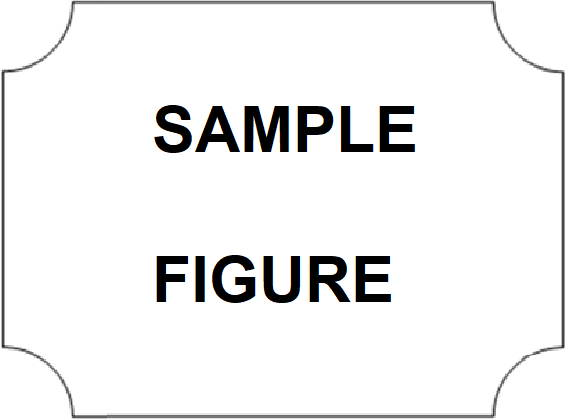
\includegraphics[width=230pt,keepaspectratio=true]{sekil7}
 % sekil7.eps: 0x0 pixel, 300dpi, 0.00x0.00 cm, bb=14 14 455 369
 \vspace{4mm}
 \caption{Example table in chapter 6.}
 \label{fig:6-1}
\end{figure}

Lorem ipsum dolor sit amet, consectetur adipiscing elit. Sed ac augue vel dui 
adipiscing placerat et nec metus. Donec bibendum sodales mollis. Cras in lacus 
justo, at vestibulum quam. Sed semper, est sit amet consectetur ornare, leo est 
lacinia velit, adipiscing elementum lectus felis at sem.

\begin{table*}
{\setlength{\tabcolsep}{14pt}
\caption{Example table in chapter 6.}
\begin{center}
\vspace{-6mm}
\begin{tabular}{cccc}
\hline\hline
Column A & Column B & Column C & Column D \\
\hline
Row A & Row A & Row A & Row A \\
Row B & Row B & Row B & Row B \\
Row C & Row C & Row C & Row C \\
\hline
\end{tabular}
\vspace{-6mm}
\end{center}
\label{tableforCh6-1}}
\end{table*}

Lorem ipsum dolor sit amet, consectetur adipiscing elit. Sed ac augue vel dui 
adipiscing placerat et nec metus. Donec bibendum sodales mollis. Cras in lacus 
justo, at vestibulum quam. Sed semper, est sit amet consectetur ornare, leo est 
lacinia velit, adipiscing elementum lectus felis at sem. Aenean hendrerit erat eu 
lacus malesuada at sodales arcu egestas. Maecenas euismod urna ut sem luctus et 
congue metus vulputate. Ut pellentesque, neque eget fringilla elementum, ligula 
massa aliquet lorem, et varius nisi lacus vel diam. Etiam vitae metus sed orci 
rutrum fringilla. Phasellus sed velit quam. Mauris vestibulum, mauris a cursus 
adipiscing, nulla est hendrerit justo, ut fringilla eros velit ut mauris.

\bibliographystyle{itubib} 
\bibliography{references}


% YÖK kararıyla özgeçmişe email gibi kişisel bilgiler yazmak yasaklanmış.
\ozgecmis{\vspace{10mm}

%\newsavebox{\mysquare}
%\savebox{\mysquare}{\textcolor{black}{\rule[2.3pt]{3.4pt}{3.4pt}}}

%\setlength{\TPHorizModule}{10pt}
%\setlength{\TPVertModule}{10pt}
%\begin{textblock}{1}(40,10)
% \begin{figure}[p]
% 
\includegraphics[scale=0.3,keepaspectratio=true]{./fig/photo}
%\end{figure}
%\end{textblock}

\textbf{Name SURNAME:} \\

%\vspace{-3mm}
%\textbf{Place and Date of Birth:} \\

%\vspace{-3mm}
%\textbf{E-Mail:} \\


\textbf{EDUCATION:} 
\vspace{-3mm}
\begin{itemize}
  \item \textbf{B.Sc.:} Graduation year, University, Faculty, Department
  \item \textbf{M.Sc.:} Graduation year, University, Faculty, Department
\end{itemize}

\textbf{PROFESSIONAL EXPERIENCE AND REWARDS:}   
\vspace{-3mm}
\begin{itemize}
  \item 1950-1956 İstanbul Technical University at the Central Laboratory of Theoretical Physics.
  \item 1953 Nobel Prize for Physics
  \item 1956 Completed Doctorate at İstanbul Technical University
\end{itemize}

\textbf{PUBLICATIONS, PRESENTATIONS AND PATENTS ON THE THESIS:} 
\vspace{-3mm}
\begin{itemize}
   \item {\bf Surname N.}, Ganapuram S., Hamidov A., Demirel, M. C., Bozkurt E., Kındap U., Newton A.
   (2007). Erasmus Mundus Scholar's Perspective On Water And Coastal
   Management Education In Europe. 
   \textit{International Congress - River Basin Management}, 
   March 22-24, 2007 Antalya, Turkey. (Presentation Instance)

   \item Satoğlu, Ş.I., Durmuşoğlu, M. B., {\bf Surname N.}, Ertay, T. A. (2010). A Mathematical Model 
   And A Heuristic Approach For Design Of The Hybrid Manufacturing Systems 
   To Facilitate One-Piece Flow, 
   \textit{International Journal of Production Research,}
   48(17), 5195-5220. (Article Instance)


   \item  {\bf Surname N.} (2013). Intelligent Digital Teaching And Learning All-In-One Machine,
   Has Projection Mechanism Whose Front End Is Connected With Supporting
   Arm, And Base Shell Provided With Panoramic Camera That Is Connected With
   Projector. Patent numarası: CN203102627-U (Patent Instance)
\end{itemize}

\newpage

\textbf{OTHER PUBLICATIONS, PRESENTATIONS AND PATENTS:} 
\vspace{-3mm}
% ---------------------------------------------------------------- %
% Fotografli ve yayin listeli (yayini varsa) ozgecmis onerilir.    %
% Fotograf ve adres sart degildir.				   %
% ---------------------------------------------------------------- %}
\end{document} 